\RequirePackage{luatex85}
\documentclass[border=8pt]{standalone}
\usepackage{tikz}
\usepackage{graphicx}
\usepackage{amsmath}
\usepackage{xcolor}
\usetikzlibrary{decorations.pathreplacing, calc, positioning, arrows.meta}

\definecolor{eqblue}{HTML}{1F4E96}
\definecolor{annotred}{HTML}{D62828}

\begin{document}
\begin{tikzpicture}[
    diag/.style={inner sep=0pt, outer sep=0pt},
    photo/.style={inner sep=0pt, outer sep=0pt, draw=black!40, line width=0.4pt},
    lbl/.style={font=\sffamily\small, align=center},
    lblbig/.style={font=\sffamily, align=center},
    arrow/.style={-{Stealth[length=5pt,width=4pt]}, draw=annotred, line width=0.7pt},
    brace/.style={decorate, decoration={brace, amplitude=5pt, raise=1pt}, draw=annotred, line width=0.6pt},
    bracedown/.style={decorate, decoration={brace, amplitude=5pt, raise=1pt, mirror}, draw=annotred, line width=0.6pt},
]

  % ------------------- TOP ROW -------------------
  % Dirac (label + photo + diagram)
  \node[photo] (dpic) at (0, 5.5) {
\includegraphics[width=1.9cm]{photos/dirac.png}};
  \node[lbl, above=1pt of dpic] {Dirac};
  \node[diag, anchor=south west] (ddiag) at (2.4, 4.0) {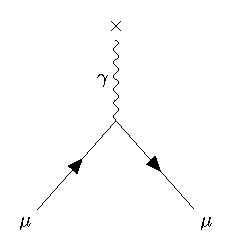
\includegraphics[height=2.7cm]{out/pdf/dirac.pdf}};
  \node[lbl, above=1pt of ddiag] {Charged,\\spin \(\tfrac{1}{2}\) particle};

  % Kinoshita
  \node[photo] (kpic) at (6.0, 5.0) {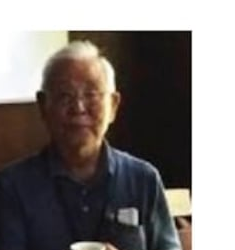
\includegraphics[width=1.9cm]{photos/kinoshita.png}};
  \node[lbl, below=1pt of kpic] {Kinoshita};
  \node[lbl, above=1pt of kpic] {12672 diagrams};
  \node[diag, anchor=south west] (kdiag) at (7.5, 4.0) {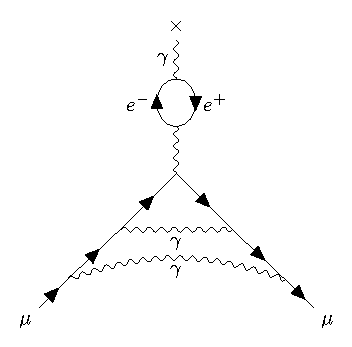
\includegraphics[height=2.7cm]{out/pdf/qed-kinoshita.pdf}};
  \node[lbl, anchor=west] at ($(kdiag.east)+(0.3,0.6)$) {Up to 10\textsuperscript{th}\\Order QED};

  % Electroweak
  \node[lbl] at (14.8, 7.2) {Electroweak};
  \node[diag, anchor=south] (eww)  at (13.5, 4.6) {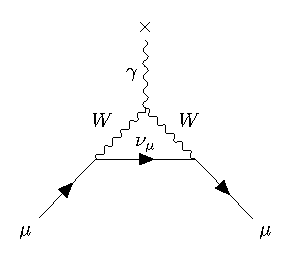
\includegraphics[height=2.4cm]{out/pdf/ew-w.pdf}};
  \node[diag, anchor=south] (ewz)  at (16.1, 4.6) {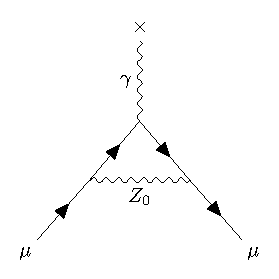
\includegraphics[height=2.4cm]{out/pdf/ew-z.pdf}};
  \node[diag, anchor=north] (ewzf) at (14.8, 4.0) {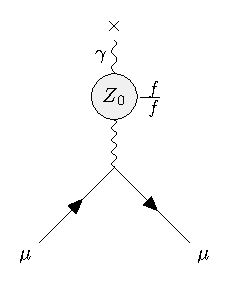
\includegraphics[height=2.4cm]{out/pdf/ew-z-fermion.pdf}};

  % ------------------- EQUATION (center) -------------------
  \node[anchor=base, font=\fontsize{36pt}{40pt}\selectfont, color=eqblue]
       (eq) at (8.0, 0) {\(g_\mu \;=\; 2.002\;331\;841\;78(126)\)};

  % Anchor points along the equation for braces (approximate x-coords).
  % Numbers are positioned in the equation; we mark digit-group bounds.
  \coordinate (eq_2)        at (4.40, -0.55);   % "2."
  \coordinate (eq_2_top)    at (4.40,  0.85);
  \coordinate (eq_002l)     at (4.85, -0.55);   % "002"
  \coordinate (eq_002r)     at (6.45, -0.55);
  \coordinate (eq_331l)     at (6.55,  0.85);   % "331"
  \coordinate (eq_331r)     at (8.05,  0.85);
  \coordinate (eq_841l)     at (8.20, -0.55);   % "841"
  \coordinate (eq_841r)     at (9.70, -0.55);
  \coordinate (eq_78l)      at (9.85,  0.85);   % "78"
  \coordinate (eq_78r)      at (10.95, 0.85);
  \coordinate (eq_126l)     at (11.10,-0.55);   % "(126)"
  \coordinate (eq_126r)     at (12.65,-0.55);

  % ------------------- BOTTOM ROW -------------------
  % Schwinger
  \node[photo] (spic) at (0, -3.6) {
\includegraphics[width=2.0cm]{photos/schwinger.png}};
  \node[lbl, above=1pt of spic] {Schwinger};
  \node[diag, anchor=north west] (sdiag) at (2.2, -2.2) {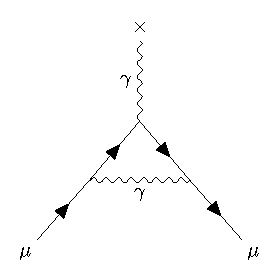
\includegraphics[height=2.7cm]{out/pdf/schwinger.pdf}};
  \node[font=\normalsize, anchor=west] (alphaeq) at ($(sdiag.east)+(0.15,0)$) {\(\dfrac{\alpha}{2\pi} = 0.00232\)};
  \node[lbl, below=1pt of sdiag] {1\textsuperscript{st} Order QED};

  % Hadronic group (top hadronic line)
  \node[lbl] at (8.7, -1.6) {Hadronic};
  \node[diag, anchor=north] (hvp)  at (7.2,  -2.0) {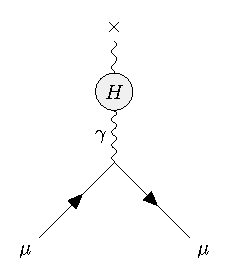
\includegraphics[height=2.4cm]{out/pdf/hadronic-vp.pdf}};
  \node[diag, anchor=north] (hvpe) at (9.0,  -2.0) {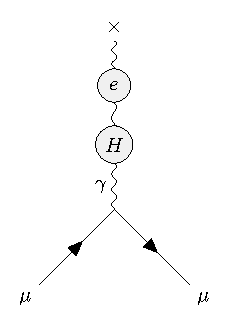
\includegraphics[height=2.4cm]{out/pdf/hadronic-vp-extra.pdf}};
  \node[diag, anchor=north] (hd)   at (10.8, -2.0) {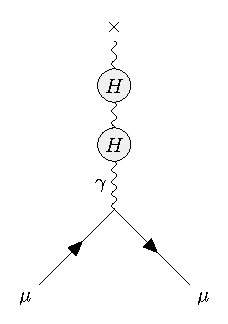
\includegraphics[height=2.4cm]{out/pdf/hadronic-double.pdf}};
  \node[lbl] (domunc) at (9.0, -5.0) {Dominant uncertainty\\in calculation};

  % Hadronic light-by-light variants (bottom row)
  \node[diag, anchor=north] (hlbls) at (8.0, -5.5) {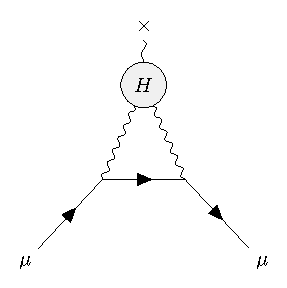
\includegraphics[height=2.4cm]{out/pdf/hadronic-lbl-small.pdf}};
  \node[diag, anchor=north] (hlbl)  at (11.0, -5.5) {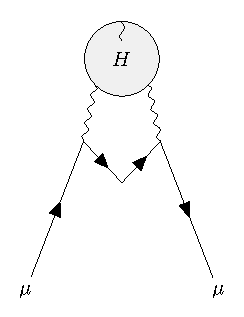
\includegraphics[height=2.4cm]{out/pdf/hadronic-lbl.pdf}};

  % Big red ?
  \node[font=\fontsize{40pt}{40pt}\selectfont\bfseries, color=annotred] (qmark) at (14.0, -4.5) {?};

  % ------------------- BRACES (red) -------------------
  % Top braces
  % "002" → Dirac (1st-order baseline; in original this slot maps to Dirac/QED)
  \draw[brace] (eq_002l) -- (eq_002r);
  % "331" → Kinoshita
  \draw[brace] (eq_331l) -- (eq_331r);
  % "78"  → Electroweak
  \draw[brace] (eq_78l)  -- (eq_78r);

  % Bottom braces
  % "002" → Schwinger
  \draw[bracedown] (eq_002l) -- (eq_002r);
  % "841" → Hadronic lower set
  \draw[bracedown] (eq_841l) -- (eq_841r);
  % "(126)" → ?
  \draw[bracedown] (eq_126l) -- (eq_126r);

  % ------------------- ARROWS (red) -------------------
  % Top row arrows: brace midpoint -> diagram
  \draw[arrow] ($(eq_002l)!0.5!(eq_002r)+(0,0.35)$)
        to[out=125, in=-90] (ddiag.south);
  \draw[arrow] ($(eq_331l)!0.5!(eq_331r)+(0,0.35)$)
        to[out=90,  in=-90] (kdiag.south);
  \draw[arrow] ($(eq_78l)!0.5!(eq_78r)+(0,0.35)$)
        to[out=60, in=-130] (ewzf.south);

  % Bottom row arrows
  \draw[arrow] ($(eq_002l)!0.5!(eq_002r)+(0,-0.45)$)
        to[out=-120, in=80] (sdiag.north east);
  \draw[arrow] ($(eq_841l)!0.5!(eq_841r)+(0,-0.45)$)
        to[out=-90, in=90]  (hvpe.north);
  \draw[arrow] ($(eq_126l)!0.5!(eq_126r)+(0,-0.45)$)
        to[out=-30, in=90]  (qmark.north);

\end{tikzpicture}
\end{document}
